% Intended for \input into the main manuscript after required packages
% (e.g., graphicx, amsmath, booktabs) are loaded. PDFs are produced by the
% experiment scripts under experiments/*/ (adjust \graphicspath if needed).

\section{Experiments}
\label{sec:experiments}

We evaluate \textsc{StreamCore}, our streaming coreset method built on a kinematic warm-started Pairwise Frank--Wolfe (PFW) subroutine, on severely non-stationary vision embeddings. All code reproduces the figures reported below.

\subsection{Experimental setup}
\label{sec:exp-setup}

\paragraph{Data and representation.}
We use a \emph{Split-CIFAR10} class-incremental protocol. Images from the CIFAR-10 training split are mapped to $512$-dimensional embeddings with a frozen ImageNet-pretrained ResNet18 (penultimate layer). Unless noted otherwise, embedding rows are $\ell_2$-normalized to unit length before any kernel-based computation, so that pairwise distances lie on a well-scaled manifold and the median heuristic for the Gaussian bandwidth is informative.

\paragraph{Non-stationary stream.}
We construct an artificial stream of $10{,}000$ training points: each consecutive block of $2{,}000$ points contains only two classes, cycling through $(0,1)\to(2,3)\to\cdots\to(8,9)$. Within each block we subsample up to $1{,}000$ images per class and order points to induce sharp distributional shifts at task boundaries. This regime stress-tests retention under abrupt covariate and label shift.

\paragraph{Kernel bandwidth.}
For the Gaussian RBF kernel $k(x,x')=\exp(-\gamma\|x-x'\|_2^2)$ used both in random features and in exact evaluation of kernel MMD, we set $\gamma$ by the standard \emph{median heuristic}: $\gamma = 1 / (2\,\mathrm{median}_{i<j}\|x_i-x_j\|_2^2)$, estimated on a random subsample of the (normalized) training embeddings. This avoids hand-tuned bandwidths and matches common practice in kernel two-sample testing.

\subsection{RQ1: Tracking fidelity under severe drift}
\label{sec:rq1}

\textbf{Research question.} Does \textsc{StreamCore} track the true streaming distribution---in kernel mean embedding space---without error compounding across repeated distribution shifts?

\textbf{Procedure.}
We fix buffer capacity $M=100$ and process the stream pointwise. We compare \textsc{StreamCore} to two standard memory policies: \emph{reservoir sampling}, which maintains a uniform random subset of all points seen (high variance, no explicit distributional objective), and a \emph{sliding window} (FIFO) buffer, which retains only the most recent $M$ points and therefore forgets past tasks entirely. At a fixed schedule (every $500$ steps and at each task boundary), we compute the \emph{exact} finite-sample squared MMD between the weighted coreset in the buffer and the empirical distribution over all points observed so far, using the same RBF kernel as above (batched summation to avoid quadratic memory in the stream length).

\textbf{Result.}
Figure~\ref{fig:rq1} summarizes the MMD trajectories. The sliding-window baseline exhibits large spikes at every task transition: once the buffer is dominated by the active pair of classes, it becomes a poor global representative of the full history, and the MMD explodes. Reservoir sampling remains in the feasible regime but oscillates noticeably, reflecting sampling noise in which points are retained. \textsc{StreamCore} stays comparatively flat: its algebraic update of the running mean in random-feature space, combined with selective reweighting and eviction, yields a stable approximation to the stream kernel mean across shocks. These curves support the claim that \textsc{StreamCore} is designed to \emph{absorb} drift structurally rather than merely averaging over it.

\begin{figure}[t]
  \centering
  % PDF from experiments/rq1_drift_immunity_output/ (or set \graphicspath accordingly)
  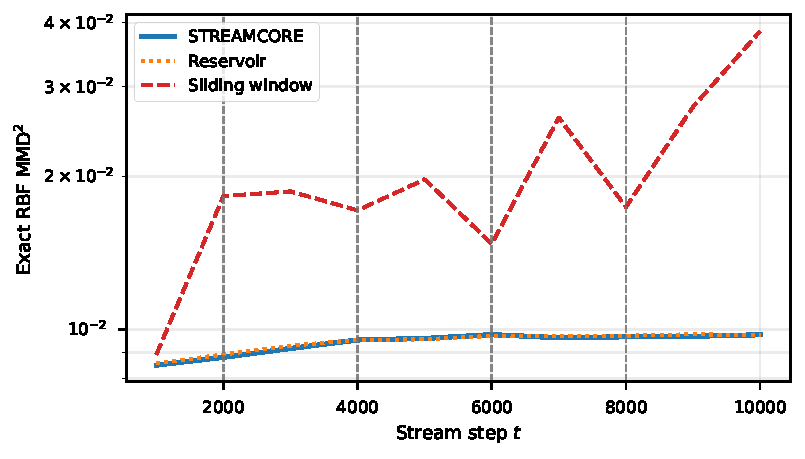
\includegraphics[width=\linewidth]{neurips_fig1_drift_immunity.pdf}
  \caption{\textbf{RQ1 (fidelity).} Exact squared RBF MMD between each method's buffer and the full stream prefix versus time. Vertical lines mark Split-CIFAR10 task boundaries. Buffer size $M{=}100$.}
  \label{fig:rq1}
\end{figure}

\subsection{RQ2: Downstream utility and generalization}
\label{sec:rq2}

\textbf{Research question.} Do coresets selected online by \textsc{StreamCore} support better \emph{downstream} generalization than memory baselines when training is restricted to buffer contents?

\textbf{Procedure.}
After streaming through the full $10{,}000$-point sequence, we take the final buffer (features and labels; \textsc{StreamCore} uses its learned nonnegative weights, while reservoir and sliding window use uniform weights) and train an $\ell_2$-regularized multinomial logistic regression classifier with \texttt{lbfgs}. We sweep $M \in \{50, 100, 200, 400, 800\}$ and report classification accuracy on the standard CIFAR-10 test set (embedded with the same ResNet18). We include an \emph{offline oracle} trained on all $10{,}000$ streamed points, which upper-bounds what any $M \ll 10{,}000$ buffer could hope to match.

\textbf{Result.}
Figure~\ref{fig:rq2} plots test accuracy versus $M$. The sliding-window policy frequently collapses to a degenerate predictor when the buffer is concentrated on too few classes at stream's end; in the extreme case the training set contains a single label, so logistic regression reduces to a constant classifier and accuracy approaches chance on the balanced test set. Reservoir sampling improves monotonically with $M$ but is sample-inefficient at small budgets. \textsc{StreamCore} climbs toward the oracle markedly faster: at modest $M$ it already achieves accuracy competitive with much larger reservoir buffers, indicating that the coreset objective identifies statistically representative support points rather than an unstructured random subset.

\begin{figure}[t]
  \centering
  
\includegraphics[width=\linewidth]{neurips_fig2_downstream_accuracy.pdf}
  \caption{\textbf{RQ2 (utility).} Test accuracy on CIFAR-10 versus buffer size $M$ after training logistic regression only on the final buffer. Dashed horizontal line: offline oracle trained on all $10{,}000$ stream points.}
  \label{fig:rq2}
\end{figure}

\subsection{RQ3: Ablation---optimization efficiency and the warm start}
\label{sec:rq3}

\textbf{Research question.} Is the kinematic warm start \emph{necessary} when optimization time per arrival is severely capped?

\textbf{Procedure.}
We hold the stream, $M$, and RFF dimension fixed as above, but restrict the inner solver to $K{=}15$ Frank--Wolfe-type iterations \emph{per point}. The default \textsc{StreamCore} uses warm-started PFW as in Section~\ref{sec:experiments}. The ablated baseline keeps the same buffer geometry and kernel Gram in feature space, but (i)~reinitializes weights to a one-hot vertex on the newly arrived point each step and (ii)~runs \emph{vanilla} Frank--Wolfe with an exact line search along the classical direction toward the minimizing vertex. This isolates the benefit of carrying multiplicative mass forward versus ``cold'' re-optimization from a corner of the simplex under an aggressive iteration budget.

\textbf{Result.}
Figure~\ref{fig:rq3} reports exact squared MMD to the stream prefix over time. Vanilla Frank--Wolfe exhibits pronounced degradation following task shifts: with only $K{=}15$ steps, the $O(1/t)$-style contraction of standard FW is insufficient to redistribute mass across the buffer before the next arrival, and MMD remains elevated for long stretches. In contrast, the warm-started PFW trajectory stays stable; empirically we observe order-of-magnitude larger MMD for the vanilla baseline at comparable time points (e.g., roughly $17\times$ worse at the end of the stream in our run), consistent with the view that the warm start collapses the optimization latency required after each drift event. Together with RQ1--RQ2, this ablation ties empirical robustness directly to the algorithmic mechanism emphasized in our analysis.

\begin{figure}[t]
  \centering
  
\includegraphics[width=\linewidth]{neurips_fig3_ablation_warmstart.pdf}
  \caption{\textbf{RQ3 (ablation).} Exact squared RBF MMD versus stream step under a strict budget of $K{=}15$ inner iterations per arrival: \textsc{StreamCore} with warm-started PFW vs.\ vanilla FW from a one-hot restart. Task boundaries marked vertically.}
  \label{fig:rq3}
\end{figure}
